{\setbeamerfont{framesubtitle}{size=\tiny}
\begin{frame}{\fe{Exercice 3 : dépendance à la température}
                 {Exercise 3: temperature-dependence}}
             {\url{https://www-cast3m.cea.fr/index.php?page=exemples&exemple=formation_pasapas_3_initial}}
  \small
  \begin{itemize}
    \item \fe{Section carrée chauffée par une source et refroidie par convection}
             {Square section with heat source and cooled by convection}\\
    \tiny
    \begin{tikzpicture}
      \node[anchor=south west,inner sep=0] (image) at (0,0)
      {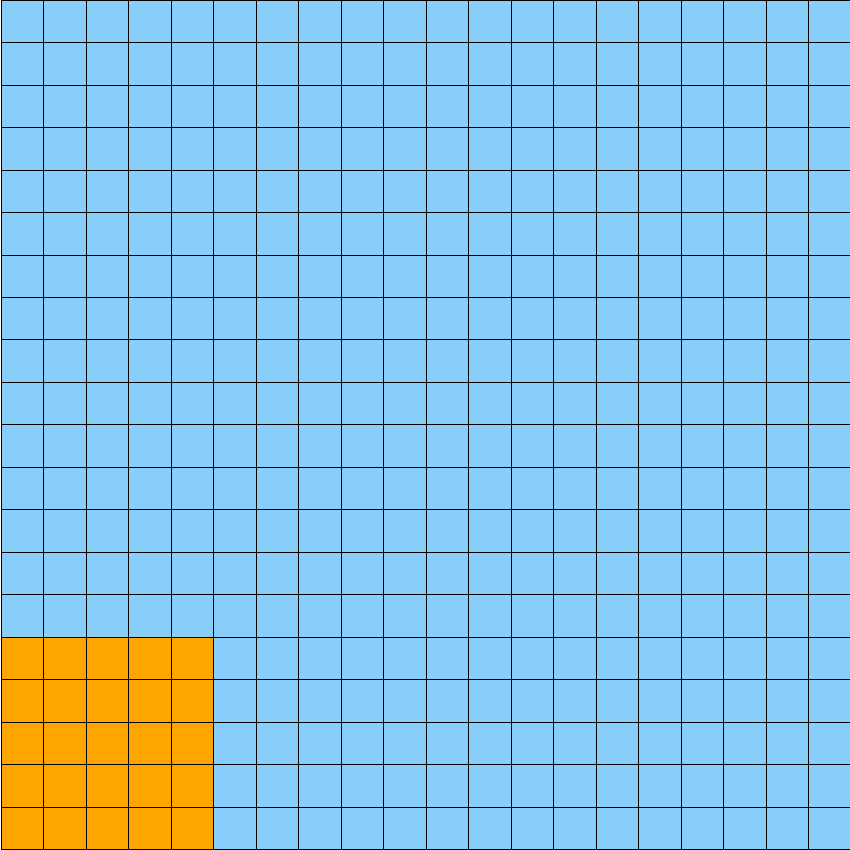
\includegraphics[height=2.5cm]{images/exo/exo_3_maillage}};
      \begin{scope}[x={(image.south east)},y={(image.north west)}]
        \draw (0.12,0.15) node {Source};
        \draw (0.5,0.5) node {$\lambda$~=~317~W/m/K};
        \draw (0.5,0.92) node {$h$~=~150~W/m$^2$/K};
        \draw[-{>[bend]}] (1.1,0.2) arc[radius=0.05, start angle=30, end angle=330];
        \draw[-{>[bend]}] (1.1,0.5) arc[radius=0.05, start angle=30, end angle=330];
        \draw[-{>[bend]}] (1.1,0.8) arc[radius=0.05, start angle=30, end angle=330];
        \draw[-{>[bend]}] (0.2,1.1) arc[radius=0.05, start angle=30, end angle=330];
        \draw[-{>[bend]}] (0.5,1.1) arc[radius=0.05, start angle=30, end angle=330];
        \draw[-{>[bend]}] (0.8,1.1) arc[radius=0.05, start angle=30, end angle=330];
      \end{scope}
    \end{tikzpicture}
    \hspace{0.1cm}
    \animategraphics[controls,loop,poster=last,height=3cm]{7}{images/exo/exo_3_temperature.}{01}{51} \hspace{0.2cm}
    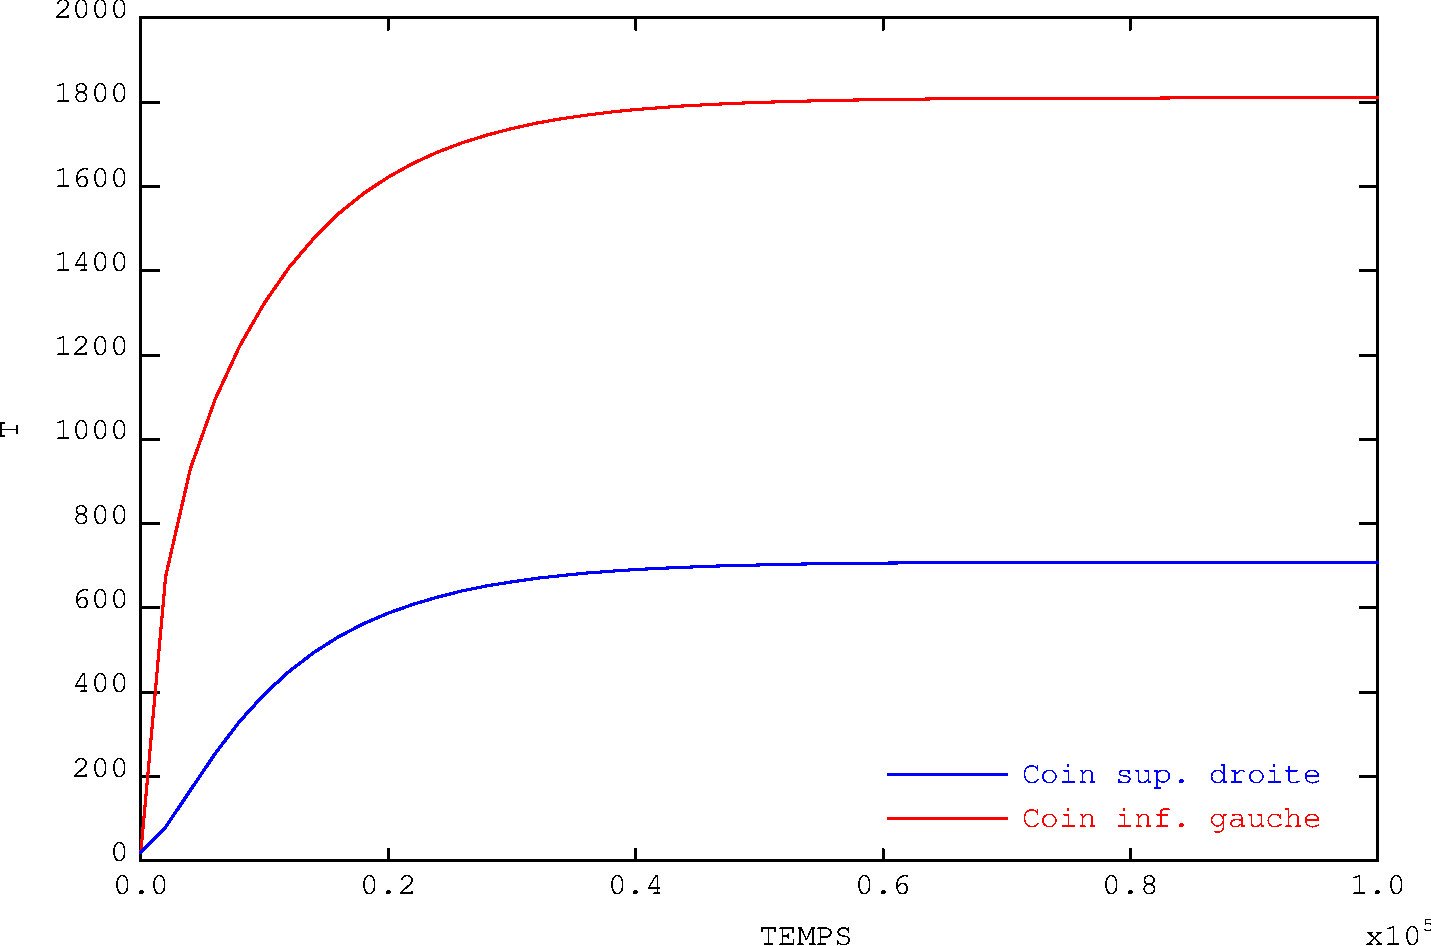
\includegraphics[height=2.6cm]{images/exo/exo_3_evol}
    \small
    \item<2-> \fe{\green{Objectif : rendre le problème variable !}}
                 {\green{Purpose: make the problem variable}}\\
    \begin{enumerate}
      \scriptsize
      \item<2-> \fe{\green{Convection fonction du temps}}
                   {\green{Time-dependent convection}}\\
        \begin{textblock*}{6cm}(7.5cm,-0.8cm)
          \tiny
          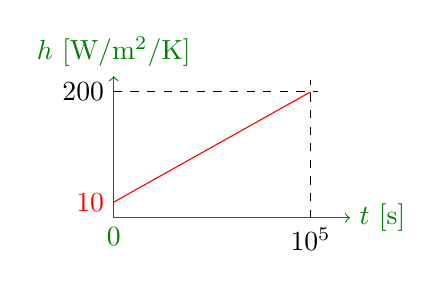
\begin{tikzpicture}
            \draw[<->,Green] (0,1.8) node (yaxis) [above] {$h$ [W/m$^2$/K]}
                          |- (3,0) node (xaxis) [right] {$t$ [s]};
            \draw[-,red] (0,0.2) node (hmin) [left] {\green{10}} -- (2.5,1.6);
            \draw[dashed] (0,1.6) node (hmax) [left] {\green{200}} -- (2.6,1.6) ;
            \draw[Green] (0,0) node[anchor=north] {0};
            \draw[dashed] (2.5,0) node (tmax) [below] {\green{10$^5$}} -- (2.5,1.75) ;
          \end{tikzpicture}
        \end{textblock*}
      \item<3-> \fe{\green{Conductivité fonction de la température}}
                   {\green{Temperature-dependent conductivity}}\\
                \green{$\lambda (T)=0.3T+200$}
      \item<4-> \fe{\green{Source fonction de la température}}
                   {\green{Temperature-dependent heat source}}\\
                \green{$q(T)=4.10^6~\tx{exp}^{-\left(\frac{T-1000}{700}\right)^2}$}
      \begin{center}
        \fe{\avous{~À vous de jouer !}}{\avous{~It's up to you!}}
      \end{center}
    \end{enumerate}
  \end{itemize}
\end{frame}
}

{\setbeamerfont{framesubtitle}{size=\tiny}
\begin{frame}{\fe{Exercice 3 : dépendance à la température}
                 {Exercise 3: temperature-dependence}}
             {\url{https://www-cast3m.cea.fr/index.php?page=exemples&exemple=formation_pasapas_3_initial}}
  \begin{itemize}
    \item \fe{Quelques objets utiles}{Some useful objects}\\
    \footnotesize
    \kw{sou~~} \fe{maillage de la source de chaleur}{heat source mesh}\\
    \kw{mosou} \fe{modèle thermique réduit sur le maillage de la source}{reduced thermal model on the heat source mesh}\\
    \normalsize
    \item \fe{Quelques opérateurs utiles}{Some useful operators}\\
    \footnotesize
    \kwr{REDU} \fe{réduction des températures sur \kw{sou}}{reduce temperatures on \kw{sou}}\\
    \kwr{SOUR} \fe{imposer une source volumique de chaleur}{impose a volume heat source}\\
    \normalsize
    \item \fe{Quelques indices utiles de la table}{Some useful table indices}\\
    \footnotesize
    \kwg{'WTABLE'.'THER\_COURANT'} \fe{températures courantes (itérations de \kwo{TRANSNON})}
                                      {current temperatures (\kwo{TRANSNON} iterations)}\\
    \kwg{'WTABLE'.'CHARGEMENT'} \fe{chargement courant}{current load}
    \normalsize
  \end{itemize}
\end{frame}
}

\begin{frame}{\fe{Exercice 3 : dépendance à la température}
                 {Exercise 3: temperature-dependence}}
             {\fe{Solution avec PERSO2}{Solution with PERSO2}}
  \footnotesize
  \begin{itemize}
    \small
    \item \fe{Utiliser des objets EVOLUTIO pour $\lambda(T)$ et $h(t)$}{Use EVOLUTIO objects for $\lambda(T)$ and $h(t)$}
    \item \fe{Utiliser la procédure \kwv{PERSO2}}{Use procedure \kwv{PERSO2}}
    \item \fe{Re-calculer la source selon la température}{Update the source as function of temperature}
    \item \fe{Écraser \kwg{'WTABLE'.'CHARGEMENT'}}{Overwrite \kwg{'WTABLE'.'CHARGEMENT'}}
  \end{itemize}
  \vspace{4.5cm}
  \scriptsize
  \begin{textblock*}{10cm}(0.3cm,-4cm)
    \fe{\emph{Programme principal}}{\emph{Main program}}
    \lstinputlisting[basicstyle=\ttfamily\tiny, language=gibiane, firstline=49, lastline=52]{dgibi/formation_pasapas_3_solution.dgibi}
    \lstinputlisting[basicstyle=\ttfamily\tiny, language=gibiane, firstline=56, lastline=59]{dgibi/formation_pasapas_3_solution.dgibi}
    \lstinputlisting[basicstyle=\ttfamily\tiny, language=gibiane, firstline=106, lastline=109]{dgibi/formation_pasapas_3_solution.dgibi}
  \end{textblock*}
  \begin{textblock*}{10cm}(6.cm,-4cm)
    \fe{\emph{\violet{Procédure PERSO2}}}{\emph{\violet{PERSO2 procedure}}}
    \lstinputlisting[basicstyle=\ttfamily\tiny, language=gibiane, firstline=67, lastline=81]{dgibi/formation_pasapas_3_solution.dgibi}
  \end{textblock*}
\end{frame}

\begin{frame}{\fe{Exercice 3 : dépendance à la température}
                 {Exercise 3: temperature-dependence}}
             {\fe{Solution avec CHARTHER}{Solution with CHARTHER}}
  \footnotesize
  \begin{itemize}
    \small
    \item \fe{Idem mais avec la procédure \kwv{CHARTHER}}{Idem but with the \kwv{CHARTHER} procedure}
    \item \fe{Pas besoin de CHARGEMEnt initial}{No need for initial load (CHARGEMEnt object)}
  \end{itemize}
  \vspace{4.5cm}
  \scriptsize
  \begin{textblock*}{10cm}(0.3cm,-4cm)
    \fe{\emph{Programme principal}}{\emph{Main program}}
    \lstinputlisting[basicstyle=\ttfamily\tiny, language=gibiane, firstline=49, lastline=52]{dgibi/formation_pasapas_3_solution.dgibi}
    \lstinputlisting[basicstyle=\ttfamily\tiny, language=gibiane, firstline=56, lastline=59]{dgibi/formation_pasapas_3_solution.dgibi}
    \lstinputlisting[basicstyle=\ttfamily\tiny, language=gibiane, firstline=147, lastline=152]{dgibi/formation_pasapas_3_solution.dgibi}
  \end{textblock*}
  \begin{textblock*}{10cm}(6.cm,-4cm)
    \fe{\emph{\violet{Procédure CHARTHER}}}{\emph{\violet{CHARTHER procedure}}}
    \lstinputlisting[basicstyle=\ttfamily\tiny, language=gibiane, firstline=84, lastline=98]{dgibi/formation_pasapas_3_solution.dgibi}
  \end{textblock*}
\end{frame}

\begin{frame}{\fe{Exercice 3 : dépendance à la température}
                 {Exercise 3: temperature-dependence}}
  \begin{itemize}
    \item \fe{Résultats}{Results}\\
    \vspace{5cm}
    \begin{textblock*}{5cm}(0.5cm,-5cm)
      \animategraphics[controls,loop,poster=last,width=5cm]{7}{images/exo/exo_3_solu_temperature.}{01}{51}
    \end{textblock*}
    \footnotesize
    \begin{textblock*}{5cm}(6.3cm,-6cm)
      \fe{Avec \kwv{PERSO2}}{With \kwv{PERSO2}}
      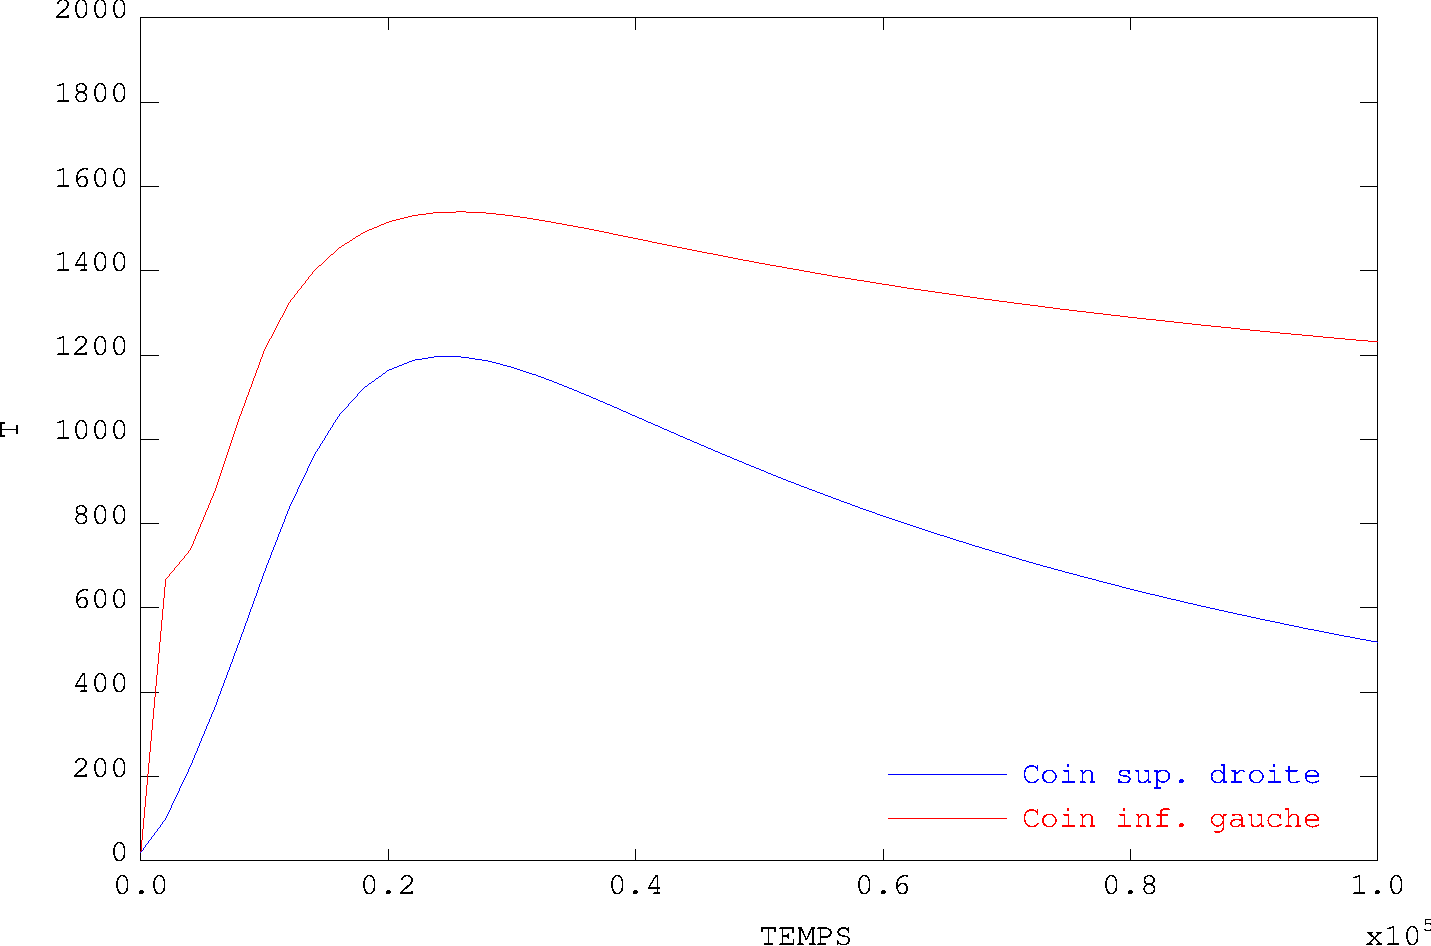
\includegraphics[width=5cm]{images/exo/exo_3_solu_evol}
    \end{textblock*}
    \begin{textblock*}{5cm}(6.3cm,-2cm)
      \fe{Avec \kwv{CHARTHER}}{With \kwv{CHARTHER}}
      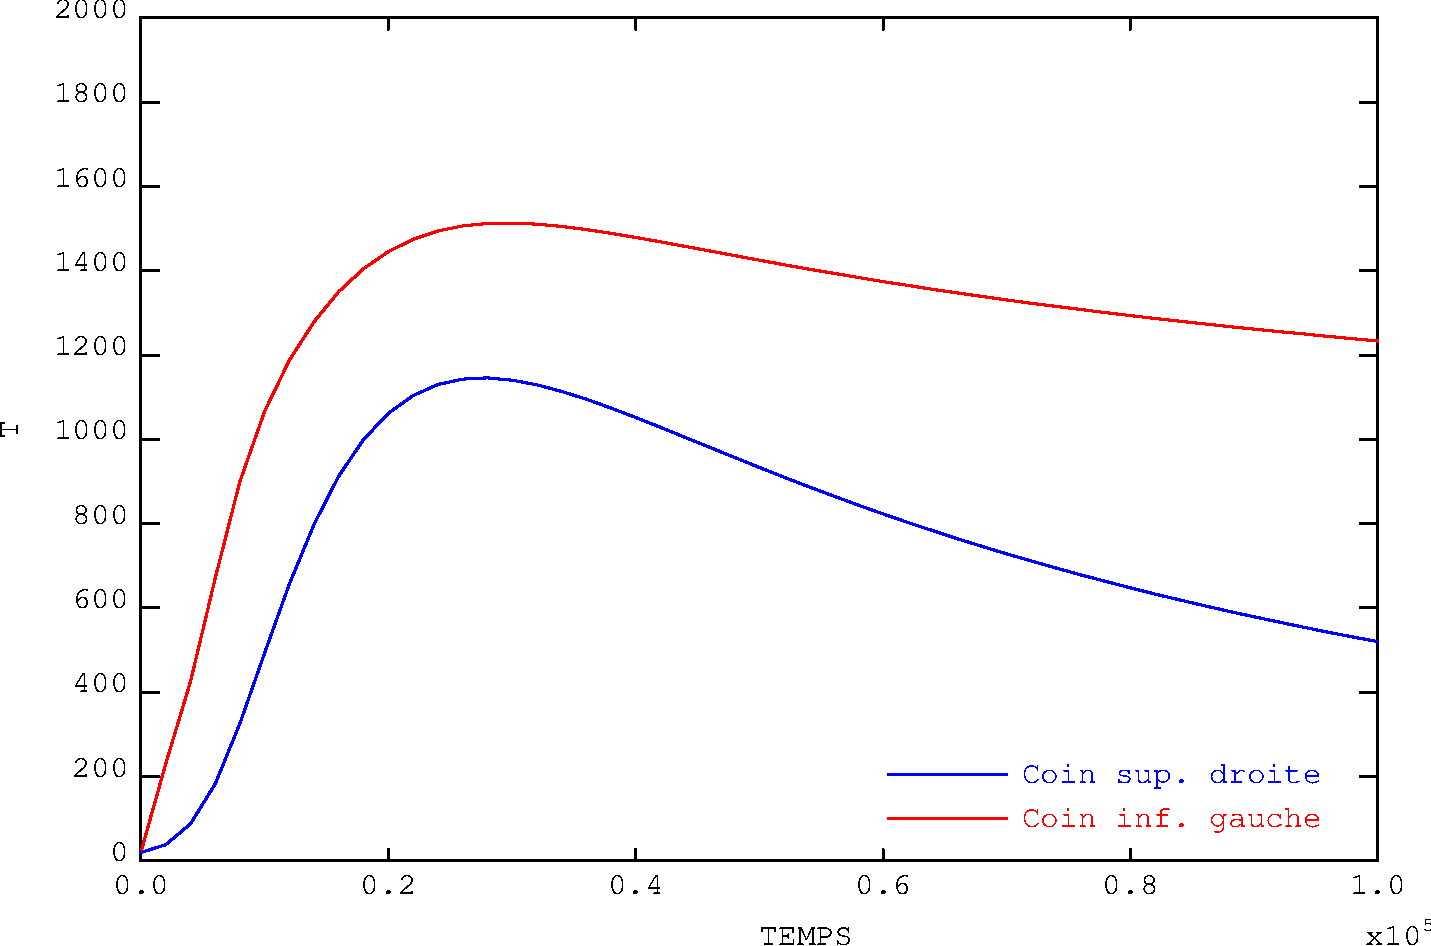
\includegraphics[width=5cm]{images/exo/exo_3_solu_bis_evol}
    \end{textblock*}
  \end{itemize}
\end{frame}
